\chapter{Figures}
\label{appendix:figures}

This appendix presents the figures generated throughout the data processing pipeline. Each figure is introduced in the order it was produced, along with a short explanation of what it represents and how it informed decisions in the pipeline.

\begin{figure}[H]
    \centering
    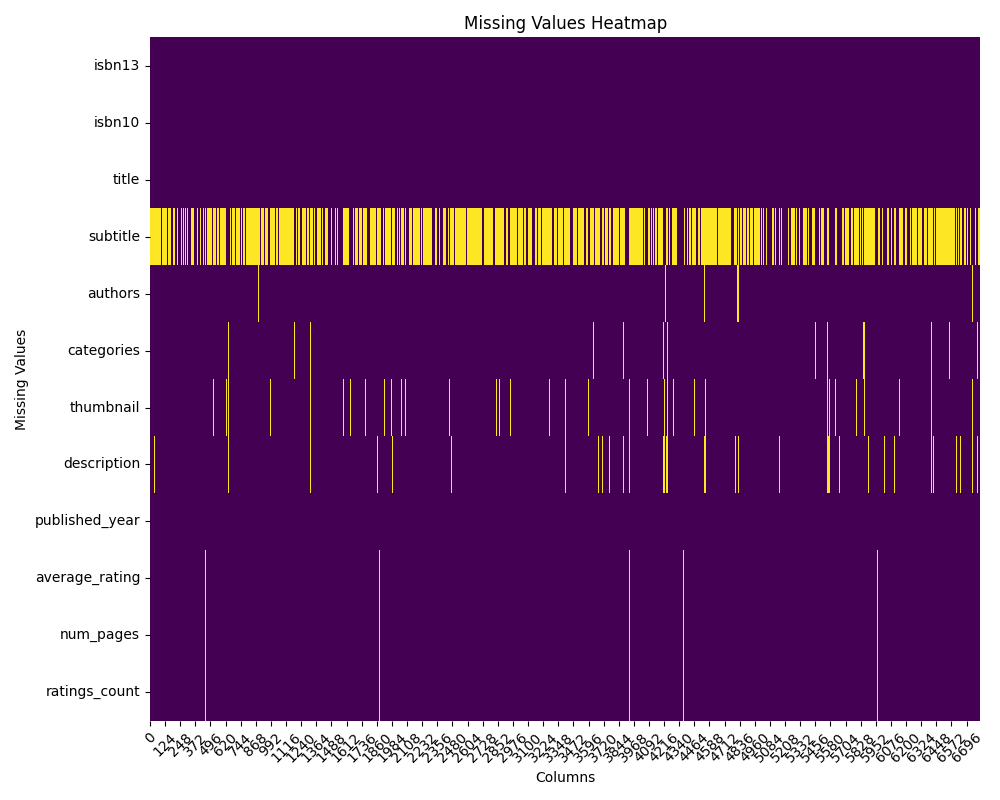
\includegraphics[width=0.9\textwidth]{figures/missing_values_heatmap.png}
    \caption{Missing Values Heatmap: Visualizes the density of missing fields in the original dataset. The heatmap highlights common gaps such as missing subtitles, authors, and thumbnails, prompting the need for augmentation.}
\end{figure}

\begin{figure}[H]
    \centering
    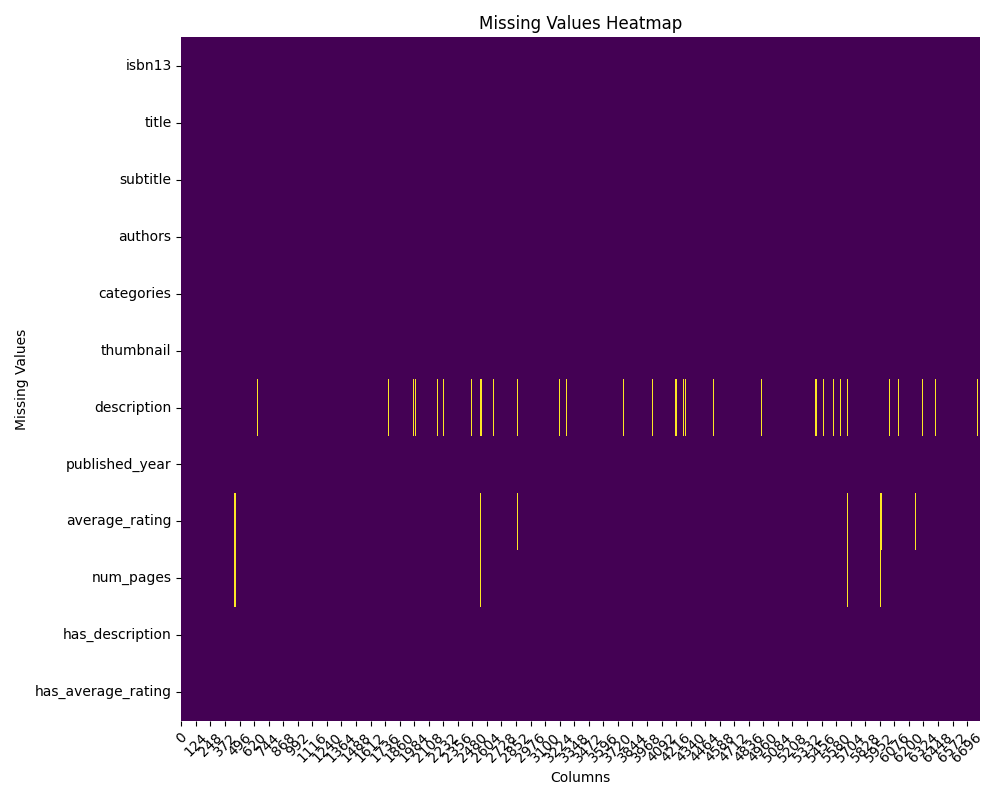
\includegraphics[width=0.9\textwidth]{figures/openlib_values_heatmap.png}
    \caption{OpenLibrary Completion Heatmap: Displays the remaining missing values after OpenLibrary augmentation. It shows improvements in coverage of fields like subtitles, page counts, and published years.}
\end{figure}

\begin{figure}[H]
    \centering
    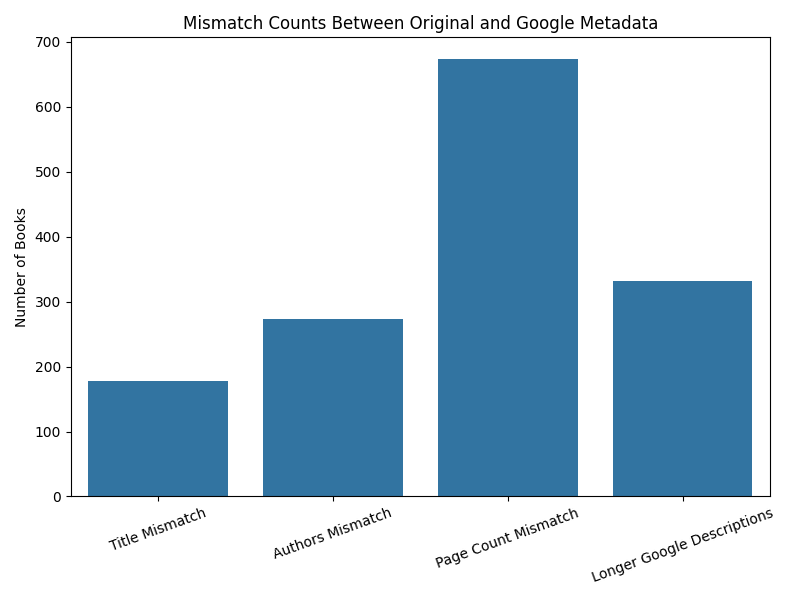
\includegraphics[width=0.9\textwidth]{figures/reexp_mismatch_counts.png}
    \caption{Metadata Conflict Counts: A bar chart showing the number of books with mismatches in title, author, or page count across sources. This justified creation of alternative metadata fields.}
\end{figure}

\begin{figure}[H]
    \centering
    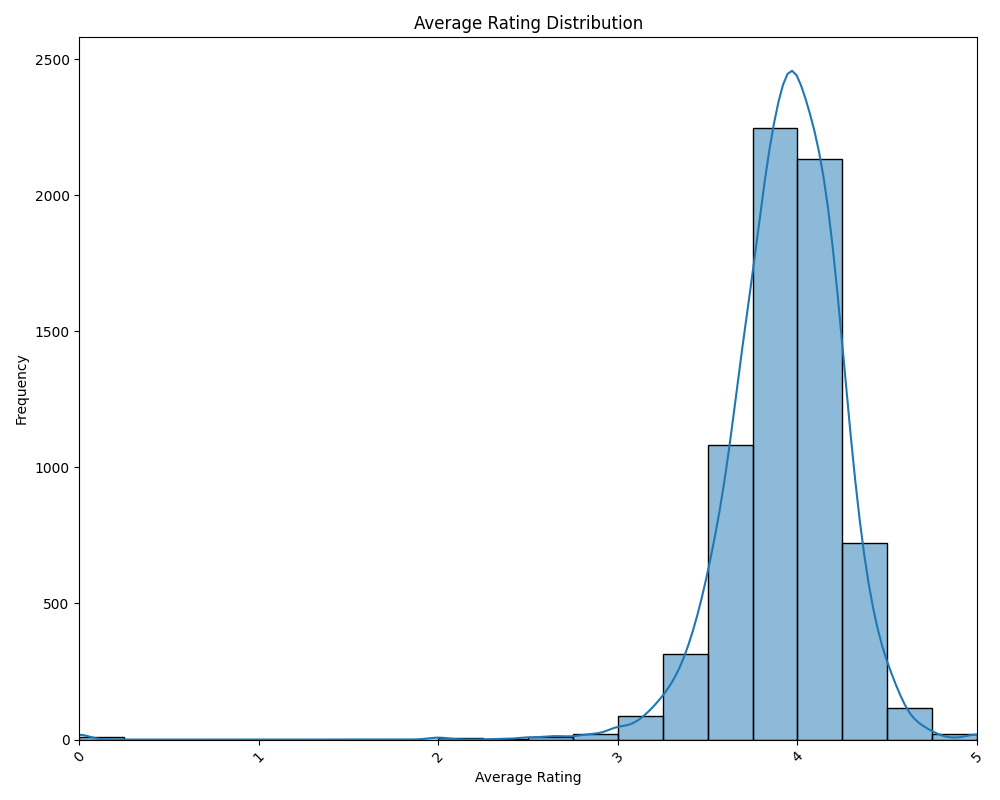
\includegraphics[width=0.9\textwidth]{figures/rating_distribution.png}
    \caption{Rating Distribution: Histogram of average book ratings. The skew toward higher ratings is typical for user-generated content and informed filter default settings.}
\end{figure}

\begin{figure}[H]
    \centering
    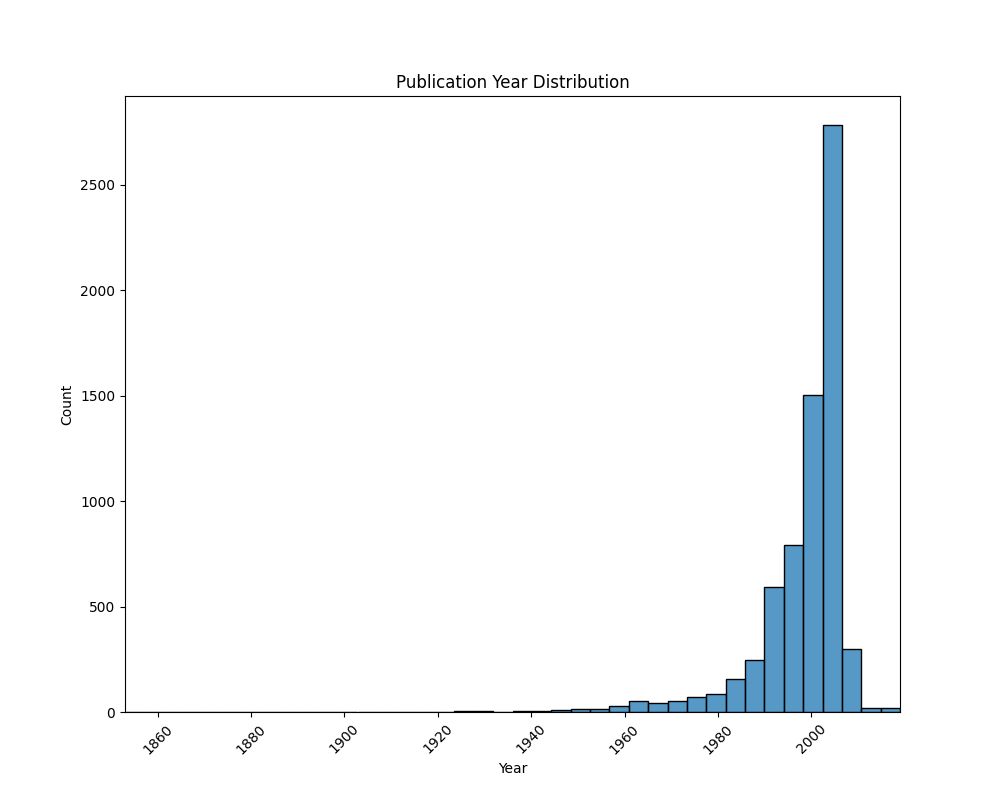
\includegraphics[width=0.9\textwidth]{figures/publication_year_distribution.png}
    \caption{Publication Year Distribution: Shows the number of books published per year. The majority are post-2000, indicating a recency bias that may impact topic coverage.}
\end{figure}

\begin{figure}[H]
    \centering
    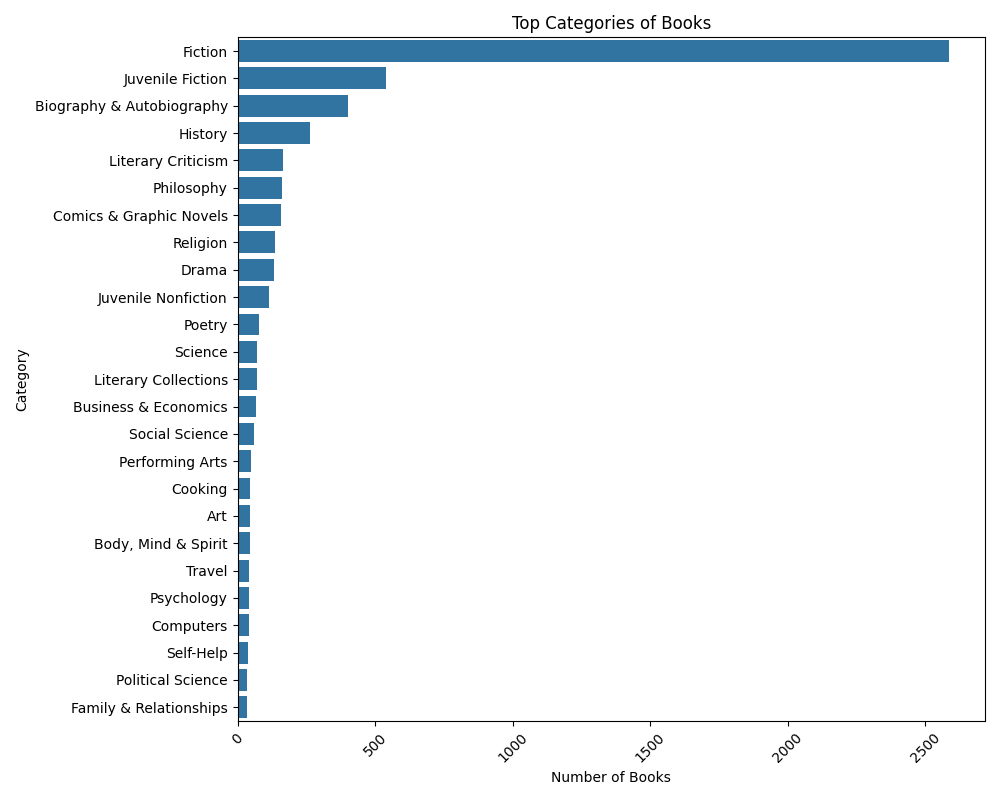
\includegraphics[width=0.9\textwidth]{figures/top_categories.png}
    \caption{Top Categories: A bar chart of the most frequent category labels in the original dataset. This informed the definition of candidate labels for zero-shot classification.}
\end{figure}

\begin{figure}[H]
    \centering
    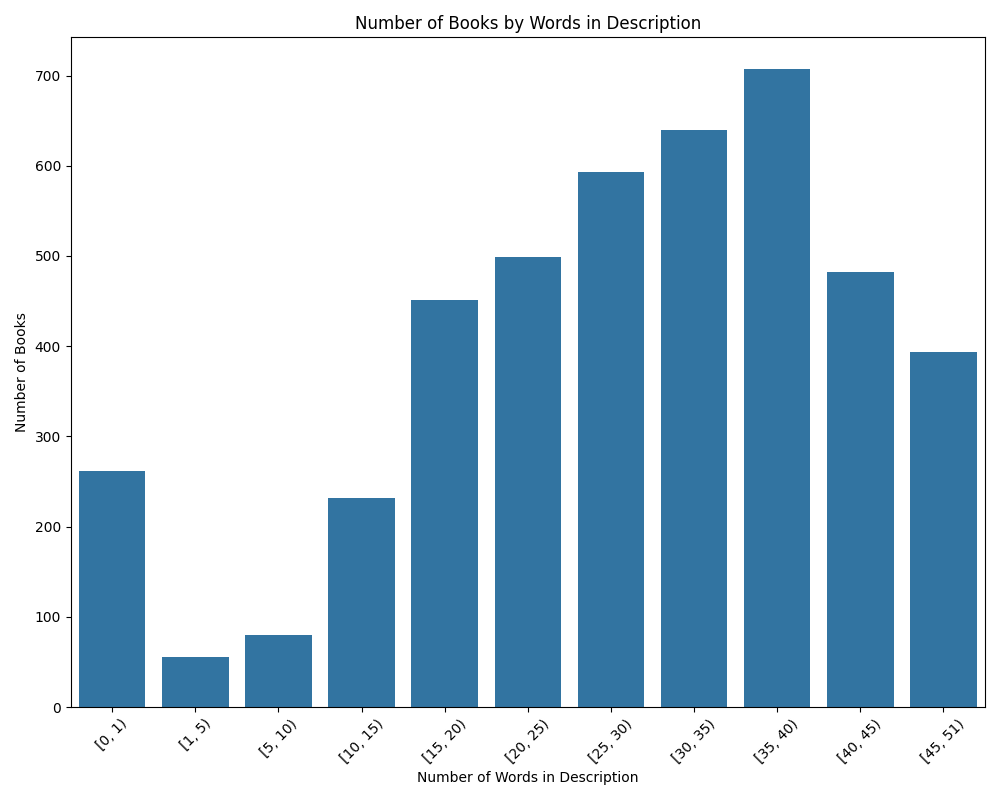
\includegraphics[width=0.9\textwidth]{figures/less_than_50_words_description.png}
    \caption{Books with Short Descriptions: Distribution of books with fewer than 50 words in their descriptions. These entries were flagged for enrichment or removal.}
\end{figure}

\begin{figure}[H]
    \centering
    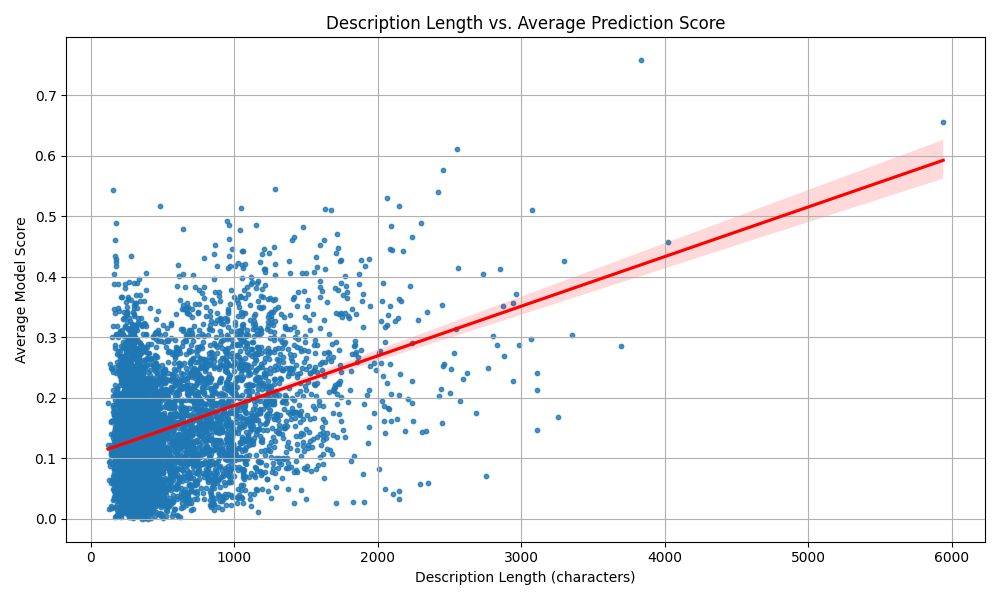
\includegraphics[width=0.9\textwidth]{figures/category_refined_description_length_vs_avg_score.png}
    \caption{Description Length vs. Confidence Score: A regression plot showing the positive correlation between description length and average model confidence. This supported the threshold of 200 characters.}
\end{figure}

\begin{figure}[H]
    \centering
    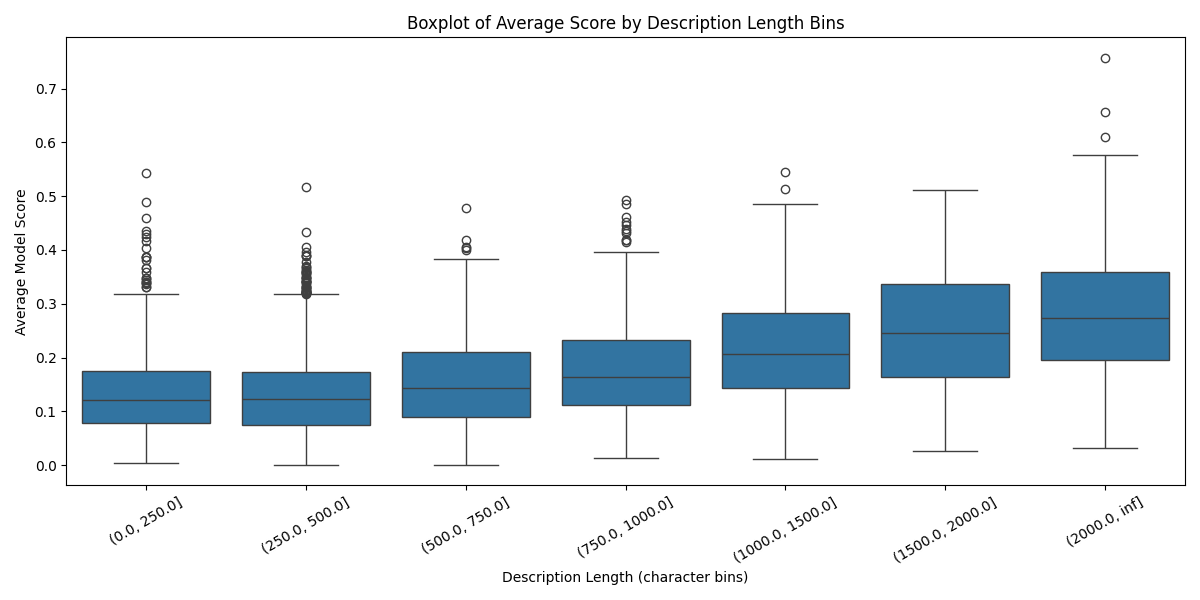
\includegraphics[width=0.9\textwidth]{figures/category_refined_avg_score_by_length_bin.png}
    \caption{Score by Length Bin: A boxplot displaying score variation across binned description lengths. Helps visualize consistency and reliability of model outputs by text richness.}
\end{figure}

\begin{figure}[H]
    \centering
    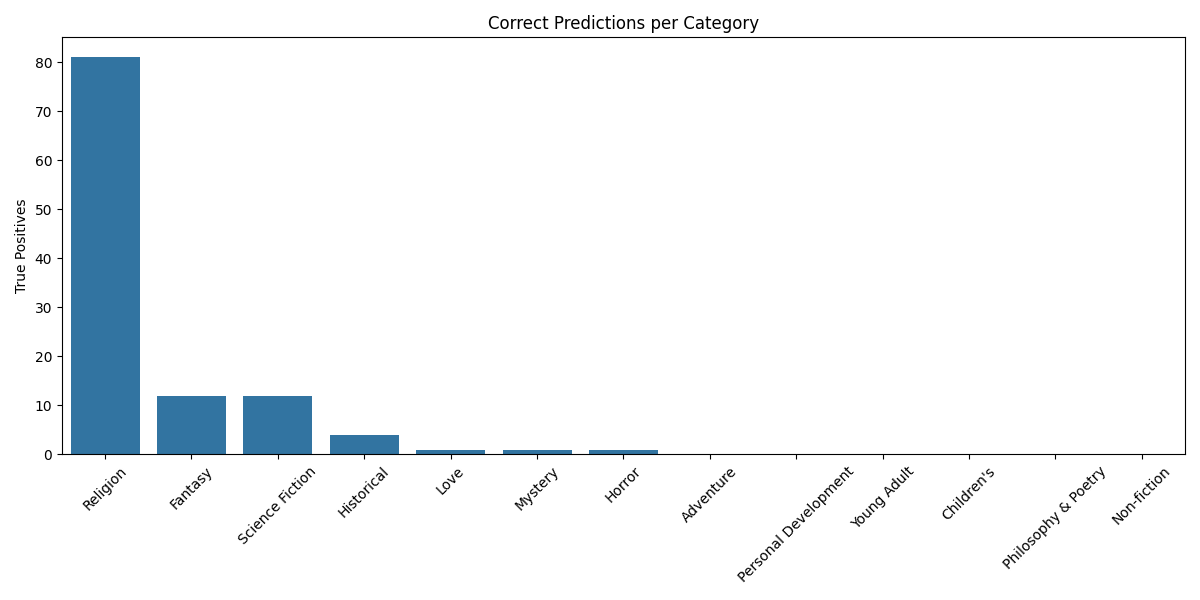
\includegraphics[width=0.9\textwidth]{figures/refine_category_prediction_matches.png}
    \caption{Prediction Matches per Category: Bar chart of true positives per category. Reflects model strength in domains like Fantasy and Love and highlights where fallback logic is critical.}
\end{figure}